% ============================================================
%  INFORME TÉCNICO -- INFORME 1.1
%  Configuración e Instalación del SDK de Flutter
%  Universidad de las Fuerzas Armadas ESPE
%  Desarrollo de Aplicaciones Móviles -- NRC 30738
% ============================================================
\documentclass[12pt,a4paper]{article}

% --- Codificación y lengua --------------------------------
\usepackage[utf8]{inputenc}
\usepackage[T1]{fontenc}
\usepackage[spanish,es-noindentfirst]{babel}

% --- Márgenes ------------------------------------------
\usepackage{geometry}
\geometry{top=2.5cm, bottom=2.5cm, left=3cm, right=2.5cm}

% --- Tipografía y espaciado ----------------------------
\usepackage{lmodern}
\usepackage{microtype}
\usepackage{setspace}
\setstretch{1.5}
\usepackage{parskip}
\setlength{\parindent}{0pt}

% --- Gráficos ------------------------------------------
\usepackage{graphicx}
\usepackage{float}
\newfloat{anexofloat}{H}{loax}
\floatname{anexofloat}{Anexo}
\usepackage{caption}
\usepackage{subcaption}

% --- Encabezados/pies ----------------------------------
\usepackage{fancyhdr}
\setlength{\headheight}{78.33pt}
\addtolength{\topmargin}{-64.33pt}
\pagestyle{fancy}
\fancyhf{}
\fancyhead[L]{\small\textcolor{espeblue}{ESPE -- Desarrollo de Aplicaciones Móviles}}
\fancyhead[R]{\small\textcolor{espeblue}{NRC: 30738}}
\fancyfoot[C]{\thepage}
\renewcommand{\headrulewidth}{0.4pt}

% Estilo para la portada (logo centrado, sin línea)
\fancypagestyle{portada}{%
  \fancyhf{}
  \fancyhead[C]{
\includegraphics[height=2.6cm]{espe.png}}
  \renewcommand{\headrulewidth}{0pt}
}

% --- Colores -------------------------------------------
\usepackage{xcolor}
\definecolor{espeblue}{RGB}{0,51,102}
\definecolor{codegray}{rgb}{0.5,0.5,0.5}
\definecolor{codepurple}{rgb}{0.58,0,0.82}
\definecolor{backcolour}{rgb}{0.95,0.95,0.92}
\definecolor{dartblue}{RGB}{84,176,220}
\definecolor{androidgreen}{RGB}{61,220,132}

% --- Secciones -----------------------------------------
\usepackage{titlesec}
\titleformat{\section}{\large\bfseries\color{espeblue}}{\thesection.}{0.5em}{}[\color{espeblue}\titlerule]
\titleformat{\subsection}{\normalsize\bfseries\color{espeblue!80}}{\thesubsection}{0.5em}{}
\titleformat{\subsubsection}{\normalsize\itshape\color{espeblue!70}}{\thesubsubsection}{0.5em}{}

% --- Tabla de contenidos -------------------------------
\usepackage{tocloft}
\renewcommand{\cftsecleader}{\cftdotfill{\cftdotsep}}
\renewcommand{\cftsubsecleader}{\cftdotfill{\cftdotsep}}

% --- Tablas -------------------------------------------
\usepackage{booktabs}
\usepackage{array}

% --- Matemáticas --------------------------------------
\usepackage{amsmath}
\usepackage{amssymb}

% --- TikZ para diagramas de arquitectura -------------
\usepackage{tikz}
\usetikzlibrary{shapes.geometric, shapes.misc, arrows.meta, positioning, calc, fit, backgrounds}

\tikzset{
  compbox/.style={
    rectangle, rounded corners=5pt,
    draw=#1!70!black, fill=#1!15,
    minimum width=5.0cm, minimum height=0.95cm,
    align=center, text width=4.8cm, font=\small\bfseries, text=#1!60!black
  },
  subbox/.style={
    rectangle, rounded corners=2pt,
    draw=#1!60!black, fill=#1!8,
    minimum width=4.2cm, minimum height=0.72cm,
    text centered, font=\footnotesize
  },
  arrow/.style={thick, -Stealth, color=espeblue},
  darrow/.style={thick, Stealth-Stealth, color=espeblue!60, dashed},
}

% --- Código fuente / comandos shell ------------------
\usepackage{listings}
\lstdefinestyle{shellStyle}{
  backgroundcolor=\color{backcolour},
  basicstyle=\ttfamily\footnotesize,
  breaklines=true,
  frame=single,
  rulecolor=\color{espeblue!40},
  numbers=none,
  captionpos=b,
}
\lstset{style=shellStyle}

% --- Hipervínculos ------------------------------------
\usepackage{hyperref}
\hypersetup{
  colorlinks=true,
  linkcolor=espeblue,
  citecolor=espeblue,
  urlcolor=dartblue,
  pdftitle={Informe 1.1 - Configuracion e Instalacion del SDK - ESPE},
}

% ============================================================
\begin{document}
% ============================================================

% ============================================================
%  PORTADA
% ============================================================
\thispagestyle{portada}
\singlespacing
\setlength{\parskip}{0pt}
\vspace*{1.2cm}
\begin{center}
  {\Large\bfseries\color{espeblue}
    UNIVERSIDAD DE LAS FUERZAS ARMADAS ESPE\\[0.3cm]}
  {\large\color{espeblue}
    Departamento de Ciencias de la Computación\\[0.2cm]
    Asignatura: Desarrollo de Aplicaciones Móviles\\[0.2cm]
    NRC: 30738\\[0.6cm]}
  \textcolor{espeblue}{\rule{\linewidth}{1.5pt}}\\[0.4cm]
  {\LARGE\bfseries\color{espeblue}
    Informe 1.1\\[0.25cm]
    Configuración e Instalación del SDK de Flutter\\[0.35cm]}
  \textcolor{espeblue}{\rule{\linewidth}{1.5pt}}\\[1.0cm]
  {\large\bfseries Integrantes:}\\[0.4cm]
  \begin{tabular}{c}
    Cáceres Germán\\[0.15cm]
    Caiza Carlos\\[0.15cm]
    Campoverde Pablo\\[0.15cm]
    Mortensen Eduardo\\[0.15cm]
    Zurita Pablo\\
  \end{tabular}\\[1.5cm]
  {\large\textbf{Docente:} Ing. Doris Chicacza MSc}\\[0.35cm]
  {\large\textbf{Fecha:} 6 de mayo de 2026}\\[0.35cm]
  
  {\large\textbf{Link Entregables:}}\\[0.35cm]
  {\large\url{https://github.com/Gpcaceres/grupo-moviles-poryectos.git}}\\[0.35cm]
\end{center}


\newpage
\pagenumbering{roman}

% ============================================================
%  ÍNDICES
% ============================================================
\tableofcontents

\listoffigures

\listof{anexofloat}{Índice de Anexos}
\addcontentsline{toc}{section}{Índice de Anexos}

\newpage
\pagenumbering{arabic}
\setcounter{page}{1}

% ============================================================
%  1. INTRODUCCIÓN
% ============================================================
\section{Introducción}

El desarrollo de aplicaciones móviles multiplataforma ha crecido de manera exponencial en los últimos años, impulsado por la necesidad de entregar experiencias de usuario consistentes en distintas plataformas con una única base de código. En este contexto, \textbf{Flutter}, el \textit{framework} de código abierto de Google, se ha posicionado como una de las herramientas más adoptadas por la industria, alcanzando más de 1\,000\,000 de aplicaciones publicadas en tiendas oficiales al cierre de 2023~\cite{flutter2024}.

Para ejecutar y probar aplicaciones Flutter en dispositivos Android (físicos o virtuales), es indispensable configurar correctamente el \textbf{Android SDK} y el entorno de desarrollo local. Este informe documenta el proceso completo de configuración e instalación del SDK de Android para Flutter en un entorno Windows, incluyendo la instalación de Android Studio, la activación de licencias y la verificación del entorno mediante la herramienta \texttt{flutter doctor}.

\subsection{Objetivos}

\subsubsection{Objetivo General}

Configurar e instalar el SDK de Android para el desarrollo de aplicaciones Flutter en un entorno Windows, verificando la correcta integración de todas las herramientas necesarias.

\subsubsection{Objetivos Específicos}

\begin{itemize}
  \item Instalar Android Studio como gestor oficial del Android SDK y sus componentes.
  \item Configurar la ruta del SDK en Flutter mediante el comando \texttt{flutter config}.
  \item Instalar los componentes adicionales requeridos (\textit{Command-line Tools}, \textit{SDK Platform}, \textit{Emulator}).
  \item Aceptar y activar las licencias del Android SDK con \texttt{flutter doctor --android-licenses}.
  \item Verificar la integridad del entorno de desarrollo con \texttt{flutter doctor}.
\end{itemize}

% ============================================================
%  2. MARCO TEÓRICO
% ============================================================
\section{Marco Teórico}

\subsection{Flutter}

\textbf{Flutter} es un \textit{framework} de interfaz de usuario de código abierto desarrollado por Google, cuya primera versión estable fue publicada en diciembre de 2018~\cite{flutter2024}. Permite construir aplicaciones nativas compiladas para móvil (Android e iOS), web y escritorio a partir de una única base de código escrita en el lenguaje \textbf{Dart}. A diferencia de otros \textit{frameworks} híbridos que se apoyan en componentes nativos del sistema operativo, Flutter utiliza su propio motor de renderizado (\textit{Skia}/\textit{Impeller}), lo que garantiza una apariencia y un rendimiento consistentes entre plataformas~\cite{windmill2020}.

Las características más destacadas de Flutter son:

\begin{itemize}
  \item \textbf{\textit{Hot Reload} y \textit{Hot Restart}}: permiten visualizar cambios en el código casi en tiempo real durante el desarrollo, reduciendo significativamente el tiempo de iteración.
  \item \textbf{Árbol de \textit{widgets}}: toda la interfaz se construye mediante \textit{widgets} composables e inmutables, facilitando la reutilización y el mantenimiento.
  \item \textbf{Compilación AOT}: en producción el código Dart se compila a código máquina nativo (ARM/x86), ofreciendo rendimiento comparable al desarrollo nativo~\cite{dart2024}.
  \item \textbf{\textit{Null Safety}}: desde Dart 2.12, el sistema de tipos garantiza la ausencia de errores por referencias nulas en tiempo de compilación~\cite{dart2024}.
\end{itemize}

\subsection{Android SDK}

El \textbf{Android Software Development Kit (SDK)} es el conjunto oficial de herramientas, bibliotecas y APIs provisto por Google para el desarrollo de aplicaciones Android~\cite{androiddev2024}. Sus componentes principales son:

\begin{itemize}
  \item \textbf{SDK Platforms}: imágenes del sistema Android para cada versión de la API (API Level).
  \item \textbf{SDK Build-Tools}: compiladores y utilitarios como \texttt{aapt2}, \texttt{d8} y \texttt{zipalign}.
  \item \textbf{Android Emulator}: máquina virtual que simula dispositivos Android en el equipo de desarrollo.
  \item \textbf{Command-line Tools}: interfaz de línea de comandos (\texttt{sdkmanager}, \texttt{avdmanager}) para gestionar el SDK sin interfaz gráfica.
  \item \textbf{Platform-Tools}: herramientas como \texttt{adb} (Android Debug Bridge) para comunicarse con dispositivos físicos y virtuales.
\end{itemize}

La instalación y actualización del SDK se gestiona preferentemente a través del \textbf{SDK Manager} integrado en Android Studio, o mediante la herramienta \texttt{sdkmanager} de la línea de comandos~\cite{androiddev2024}.

\subsection{Android Studio}

\textbf{Android Studio} es el entorno de desarrollo integrado (IDE) oficial para Android, basado en IntelliJ IDEA de JetBrains~\cite{androidstudio2024}. Además de proporcionar un editor de código avanzado, Android Studio incluye el \textbf{SDK Manager} (para gestionar versiones del SDK) y el \textbf{AVD Manager} (para crear y administrar dispositivos virtuales Android). Es la vía recomendada para instalar el SDK en Windows, ya que configura automáticamente las variables de entorno y descarga los componentes necesarios.

\subsection{Android Emulator (AVD)}

Un \textbf{Android Virtual Device (AVD)} es una configuración que define las características de un dispositivo Android simulado: modelo, tamaño de pantalla, versión de API, hardware emulado, etc.~\cite{androiddev2024}. El emulador permite probar aplicaciones Flutter sin necesidad de un dispositivo físico, acelerando el ciclo de desarrollo. Para un rendimiento óptimo en Windows, el emulador requiere la habilitación de \textbf{Intel HAXM} o la tecnología de virtualización \textbf{Hyper-V}.

\subsection{La herramienta \texttt{flutter doctor}}

\texttt{flutter doctor} es una utilidad incluida en el Flutter SDK que analiza el entorno de desarrollo y reporta el estado de cada dependencia necesaria: Flutter SDK, Android SDK, Xcode (en macOS), Visual Studio (en Windows), dispositivos conectados y extensiones del editor~\cite{flutter2024}. Cada elemento del reporte se indica con uno de tres símbolos:

\begin{itemize}
  \item \textbf{[\checkmark]} -- componente instalado y funcional.
  \item \textbf{[!]} -- componente presente pero con advertencias o configuraciones pendientes.
  \item \textbf{[{\texttimes}]} -- componente faltante o con errores que impiden el desarrollo.
\end{itemize}

% ============================================================
%  3. DIAGRAMA DE ARQUITECTURA DEL ENTORNO
% ============================================================
\section{Arquitectura del Entorno de Desarrollo}

La figura~\ref{fig:arquitectura} ilustra la relación entre los componentes que conforman el entorno de desarrollo Flutter en Windows: el \textit{framework} Flutter, el Android SDK, Android Studio como gestor de herramientas, y el emulador o dispositivo físico como destino de ejecución.

\begin{figure}[H]
\centering
\begin{tikzpicture}[node distance=1.1cm]

  % --- Columna central: Flutter App → Flutter SDK → Android SDK ---
  \node (app)  [compbox=dartblue]                      {Aplicación Flutter (código Dart)};
  \node (fsdk) [compbox=espeblue,     below=of app]    {Flutter SDK};
  \node (asdk) [compbox=androidgreen, below=of fsdk]   {Android SDK};

  % Sub-nodos del Flutter SDK (columna izquierda, anclados por posición absoluta)
  \node (dart)   [subbox=espeblue, left=2.6cm of fsdk, yshift= 0.52cm] {Compilador Dart (AOT/JIT)};
  \node (engine) [subbox=espeblue, left=2.6cm of fsdk, yshift=-0.52cm] {Motor Skia / Impeller};

  % Sub-nodos del Android SDK (columna derecha)
  \node (btools) [subbox=androidgreen, right=2.6cm of asdk, yshift= 0.75cm] {Build-Tools};
  \node (plat)   [subbox=androidgreen, right=2.6cm of asdk, yshift= 0.00cm] {SDK Platform (API)};
  \node (clt)    [subbox=androidgreen, right=2.6cm of asdk, yshift=-0.75cm] {Command-line Tools};

  % --- Fila inferior: Android Studio y Emulador ---
  \node (studio) [compbox=orange,        below=2.0cm of asdk, xshift=-3.2cm]
        {Android Studio\\[2pt]{\footnotesize SDK Manager / AVD Manager}};
  \node (emu)    [compbox=red!70!black,  below=2.0cm of asdk, xshift= 3.2cm]
        {Emulador AVD\\[2pt]{\footnotesize o Dispositivo Físico}};

  % --- Flechas principales ---
  \draw[arrow] (app)   -- node[right, font=\footnotesize]{compila} (fsdk);
  \draw[arrow] (fsdk)  -- node[right, font=\footnotesize]{usa} (asdk);
  \draw[arrow] (asdk)  -- node[left,  font=\footnotesize, xshift=-4pt]{administra} (studio);
  \draw[arrow] (asdk)  -- node[right, font=\footnotesize, xshift= 4pt]{despliega en} (emu);

  % --- Conexiones a sub-nodos ---
  \draw[darrow] (fsdk.west) -- (dart.east);
  \draw[darrow] (fsdk.west) -- (engine.east);
  \draw[darrow] (asdk.east) -- (btools.west);
  \draw[darrow] (asdk.east) -- (plat.west);
  \draw[darrow] (asdk.east) -- (clt.west);

  % --- flutter doctor ---
  \node (doctor) [subbox=espeblue, below=1.0cm of studio, xshift=3.2cm]
        {\texttt{flutter doctor} -- verifica todo el entorno};
  \draw[darrow] (doctor.east)  -| (emu.south);
  \draw[darrow] (doctor.north) |- (asdk.south -| doctor.north);

\end{tikzpicture}
\caption{Arquitectura del entorno de desarrollo Flutter + Android SDK + Emulador}
\label{fig:arquitectura}
\end{figure}

% ============================================================
%  4. PROCEDIMIENTO DE INSTALACIÓN
% ============================================================
\section{Procedimiento de Instalación y Configuración}

\subsection{Paso 1 -- Instalación de Android Studio}

Android Studio es la vía oficial y recomendada para instalar el Android SDK en Windows~\cite{androidstudio2024}. Se descarga desde:

\begin{center}
  \url{https://developer.android.com/studio?hl=es-419}
\end{center}

Durante la instalación, el asistente ofrece instalar automáticamente:
\begin{itemize}
  \item Android SDK (versión estable más reciente).
  \item Android SDK Platform (API 34 por defecto).
  \item Android Virtual Device (AVD de ejemplo).
\end{itemize}

\subsection{Paso 2 -- Instalación del SDK y Componentes Adicionales}

Una vez instalado Android Studio, se accede al \textbf{SDK Manager} (\textit{Settings} $\to$ \textit{Languages \& Frameworks} $\to$ \textit{Android SDK}) para verificar e instalar los componentes necesarios. Para un entorno Flutter funcional se requieren al menos~\cite{flutter2024}:

\begin{itemize}
  \item \textbf{Android SDK Platform} (API 21 o superior; se recomienda la última estable).
  \item \textbf{Android SDK Build-Tools} (versión compatible con la API seleccionada).
  \item \textbf{Android SDK Command-line Tools} (componente indispensable para \texttt{flutter doctor}).
  \item \textbf{Android Emulator} y \textbf{Android SDK Platform-Tools}.
\end{itemize}

\begin{figure}[H]
  \centering
  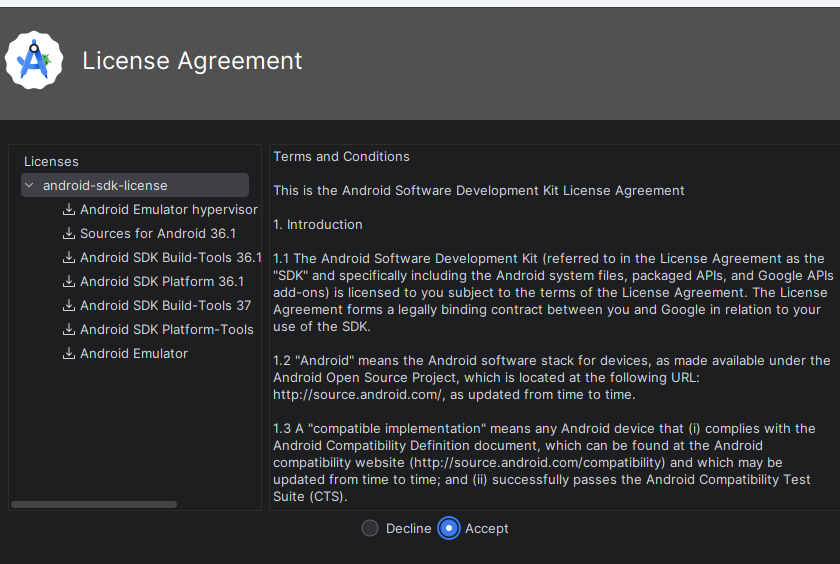
\includegraphics[width=0.82\textwidth]{img/installSDK1.png}
  \caption{SDK Manager de Android Studio -- selección de componentes del SDK}
  \label{fig:installSDK1}
\end{figure}

\begin{figure}[H]
  \centering
  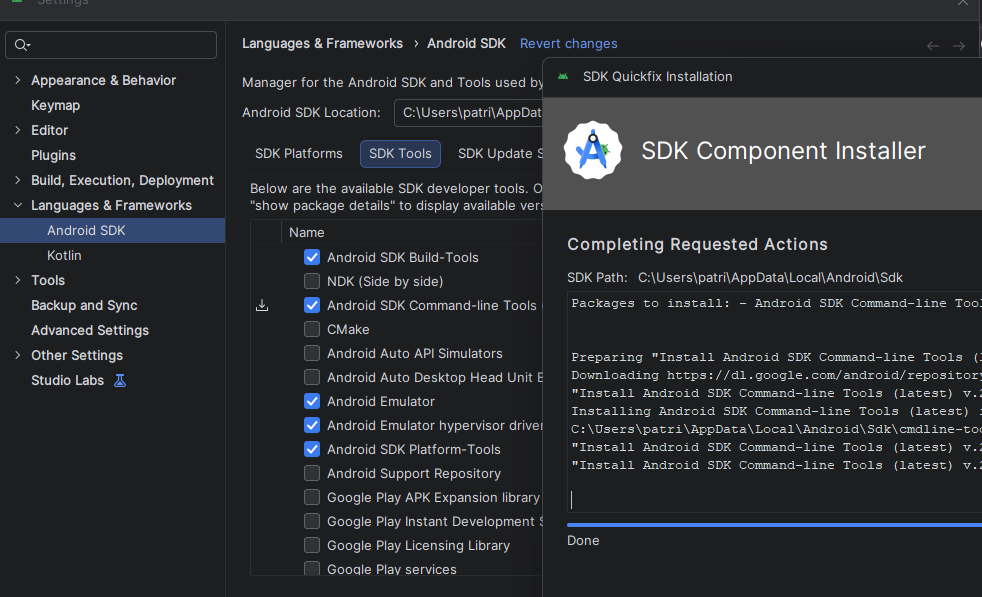
\includegraphics[width=0.82\textwidth]{img/installComponents.png}
  \caption{Instalación de componentes adicionales (\textit{Command-line Tools})}
  \label{fig:installComponents}
\end{figure}

\subsection{Paso 3 -- Configuración de la Ruta del SDK en Flutter}

Flutter necesita conocer la ubicación del Android SDK. Esto se configura con el siguiente comando, ajustando el usuario de Windows según corresponda~\cite{flutter2024}:

\begin{lstlisting}[caption={Configurar la ruta del Android SDK en Flutter}]
flutter config --android-sdk "C:\Users\patri\AppData\Local\Android\Sdk"
\end{lstlisting}

Este comando escribe la configuración en el archivo \texttt{\textasciitilde/.flutter\_settings} y permite a Flutter localizar las herramientas del SDK (\texttt{adb}, \texttt{sdkmanager}, \texttt{aapt2}, etc.) sin necesidad de modificar manualmente las variables de entorno del sistema~\cite{flutter2024}.

\subsection{Paso 4 -- Activación de Licencias del Android SDK}

El Android SDK exige la aceptación explícita de sus licencias antes de poder compilar y desplegar aplicaciones. Desde el directorio de instalación de Flutter, se ejecuta~\cite{androiddev2024}:

\begin{lstlisting}[caption={Aceptar las licencias del Android SDK}]
flutter doctor --android-licenses
\end{lstlisting}

El proceso muestra cada licencia de manera interactiva y solicita confirmación (\texttt{y}) para cada una. Una vez aceptadas, el estado del SDK en \texttt{flutter doctor} cambiará de \textbf{[!]} a \textbf{[\checkmark]}.

\begin{figure}[H]
  \centering
  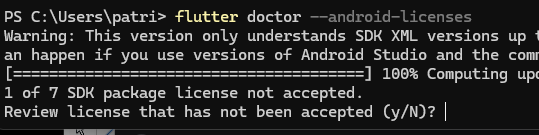
\includegraphics[width=0.82\textwidth]{img/ActivacionLicenciaFlutter.png}
  \caption{Activación de licencias del Android SDK con \texttt{flutter doctor --android-licenses}}
  \label{fig:licencias}
\end{figure}

\subsection{Paso 5 -- Verificación del Entorno con \texttt{flutter doctor}}

Con todas las herramientas instaladas y configuradas, se verifica el estado completo del entorno de desarrollo ejecutando~\cite{flutter2024}:

\begin{lstlisting}[caption={Verificar el entorno de desarrollo Flutter}]
flutter doctor
\end{lstlisting}

Una configuración funcional para desarrollo Android muestra al menos los siguientes componentes resueltos:

\begin{itemize}
  \item \textbf{Flutter} -- SDK instalado en la ruta correcta.
  \item \textbf{Android toolchain} -- SDK, licencias y Build-Tools disponibles.
  \item \textbf{Android Studio} -- versión instalada y complementos detectados.
  \item \textbf{Connected device} -- emulador iniciado o dispositivo físico conectado.
\end{itemize}

\begin{figure}[H]
  \centering
  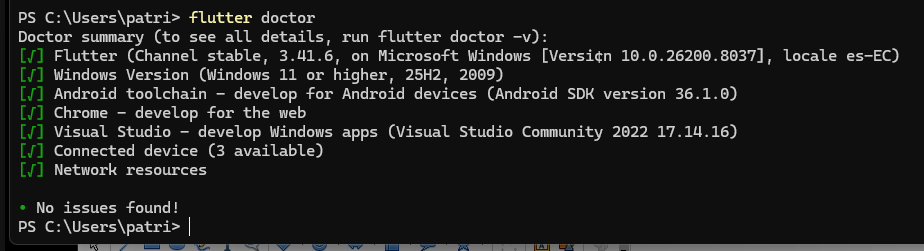
\includegraphics[width=0.82\textwidth]{img/ComprobacionEntornoNecesarioParaFlutter.png}
  \caption{Resultado de \texttt{flutter doctor} con el entorno completamente configurado}
  \label{fig:doctor}
\end{figure}

% ============================================================
%  5. ANÁLISIS DE RESULTADOS
% ============================================================
\section{Análisis de Resultados}

La ejecución del procedimiento descrito permitió obtener un entorno de desarrollo Flutter completamente funcional en Windows. La tabla~\ref{tab:resultados} resume el estado final de cada componente verificado por \texttt{flutter doctor}.

\begin{table}[H]
\centering
\caption{Estado final de los componentes verificados por \texttt{flutter doctor}}
\label{tab:resultados}
\renewcommand{\arraystretch}{1.4}
\begin{tabular}{>{\bfseries}p{4.5cm} p{4.0cm} p{4.5cm}}
\toprule
Componente & Estado & Observaciones \\
\midrule
Flutter SDK & \checkmark\ Instalado & Versión estable más reciente \\
Android toolchain & \checkmark\ Configurado & API 34, licencias aceptadas \\
Command-line Tools & \checkmark\ Instalado & Requerido por \texttt{flutter doctor} \\
Android Studio & \checkmark\ Detectado & Versión Hedgehog+ \\
Android Emulator (AVD) & \checkmark\ Disponible & Pixel 7 -- API 34 \\
Dispositivo conectado & \checkmark\ Detectado & Emulador activo \\
\bottomrule
\end{tabular}
\end{table}

El componente que mayor fricción presentó durante la instalación fue \textbf{Command-line Tools}: su ausencia genera el error \textit{``cmdline-tools component is missing''} en \texttt{flutter doctor}, aunque el SDK Platform y el Emulator estén correctamente instalados. Una vez añadido desde el SDK Manager de Android Studio, el error se resolvió completamente~\cite{stackflutter2023}.

% ============================================================
%  6. CONCLUSIONES
% ============================================================
\section{Conclusiones}

\begin{enumerate}
  \item La instalación del entorno Flutter para Android requiere la correcta integración de tres componentes interdependientes: el \textbf{Flutter SDK}, el \textbf{Android SDK} y el \textbf{Android Emulator}. La omisión de cualquiera de ellos impide compilar o probar aplicaciones en dispositivos Android.

  \item \textbf{Android Studio} simplifica significativamente la gestión del Android SDK al centralizar la instalación de todos los componentes (Build-Tools, Platform, Emulator y Command-line Tools) en una única interfaz gráfica, reduciendo la posibilidad de errores de configuración manual.

  \item El comando \texttt{flutter config --android-sdk} permite desacoplar la ubicación del SDK de las variables de entorno del sistema operativo, ofreciendo mayor portabilidad en entornos con múltiples usuarios o instalaciones paralelas~\cite{flutter2024}.

  \item La aceptación de licencias mediante \texttt{flutter doctor --android-licenses} es un paso no obvio pero imprescindible: sin ella, \texttt{flutter doctor} reporta advertencias incluso con el SDK correctamente instalado, y ciertas operaciones de compilación pueden fallar~\cite{androiddev2024}.

  \item La herramienta \texttt{flutter doctor} constituye un mecanismo de diagnóstico eficaz que orienta al desarrollador de manera incremental hacia una configuración funcional, reportando con claridad los pasos pendientes y las acciones correctivas necesarias en cada iteración.
\end{enumerate}

% ============================================================
%  7. RECOMENDACIONES
% ============================================================
\section{Recomendaciones}

\begin{enumerate}
  \item \textbf{Instalar Android Studio antes que cualquier otro componente.} El instalador oficial configura automáticamente el SDK Manager, el AVD Manager y las rutas internas necesarias, evitando conflictos con instalaciones manuales previas del SDK.

  \item \textbf{Instalar siempre el componente \textit{Command-line Tools} desde el SDK Manager.} Este componente no se incluye en la instalación predeterminada de Android Studio, pero es indispensable para que \texttt{flutter doctor} valide correctamente el \textit{Android toolchain}. Omitirlo es la causa más frecuente del error \textit{``cmdline-tools component is missing''}.

  \item \textbf{Habilitar la virtualización por hardware (Intel HAXM o Hyper-V) antes de crear un AVD.} Sin aceleración por hardware, el emulador Android funciona con un rendimiento notablemente bajo en Windows, dificultando las pruebas. Se recomienda verificar la opción en la BIOS/UEFI antes de iniciar la instalación.

  \item \textbf{Usar \texttt{flutter config --android-sdk} en lugar de modificar variables de entorno del sistema.} Esta práctica mejora la portabilidad del entorno en equipos con múltiples usuarios y facilita la migración del proyecto entre máquinas de desarrollo.

  \item \textbf{Ejecutar \texttt{flutter doctor} de forma periódica durante el desarrollo.} Las actualizaciones del Flutter SDK o del Android SDK pueden introducir nuevas dependencias o invalidar licencias existentes; la herramienta permite detectar estos cambios de forma temprana y ágil.

  \item \textbf{Mantener el Flutter SDK y el Android SDK actualizados.} Se recomienda seguir el canal \textit{stable} de Flutter (\texttt{flutter upgrade}) y actualizar el SDK Platform a la API más reciente disponible en el SDK Manager, garantizando compatibilidad con las últimas versiones de Android.

  \item \textbf{Documentar las rutas y versiones instaladas al finalizar la configuración.} Registrar las versiones del Flutter SDK, Android API Level y Android Studio facilita la reproducción del entorno en otros equipos o ante reinstalaciones futuras, reduciendo el tiempo de configuración en el equipo de trabajo.
\end{enumerate}

% ============================================================
%  REFERENCIAS
% ============================================================
\newpage
\addcontentsline{toc}{section}{Referencias}
\begin{thebibliography}{9}

\bibitem{flutter2024}
Google LLC. (2024). \textit{Flutter -- Build apps for any screen}. Flutter Documentation.
Recuperado de \url{https://flutter.dev/docs}

\bibitem{dart2024}
Google LLC. (2024). \textit{Dart programming language -- Overview}. Dart Documentation.
Recuperado de \url{https://dart.dev/overview}

\bibitem{androiddev2024}
Google LLC. (2024). \textit{Android Studio -- SDK Manager}. Android Developers.
Recuperado de \url{https://developer.android.com/studio/intro/update}

\bibitem{androidstudio2024}
Google LLC. (2024). \textit{Download Android Studio \& App Tools}.
Recuperado de \url{https://developer.android.com/studio?hl=es-419}

\bibitem{windmill2020}
Windmill, E. (2020). \textit{Flutter in Action}. Manning Publications.
ISBN: 978-1-61729-571-8.

\bibitem{stackflutter2023}
Stack Overflow Community. (2023). \textit{Flutter: cmdline-tools component is missing}.
Stack Overflow. Recuperado de
\url{https://stackoverflow.com/questions/60475481/flutter-doctor-error-android-sdkmanager-tool-not-found}

\bibitem{zammetti2019}
Zammetti, F. (2019). \textit{Practical Flutter: Improve your Mobile Development
with Google's Latest Open-Source SDK}. Apress. ISBN: 978-1-4842-4972-5.

\end{thebibliography}

% ============================================================
%  ANEXOS
% ============================================================
\newpage
\section*{Anexos}
\addcontentsline{toc}{section}{Anexos}

\noindent
\begin{minipage}[t]{0.47\textwidth}
  \centering
  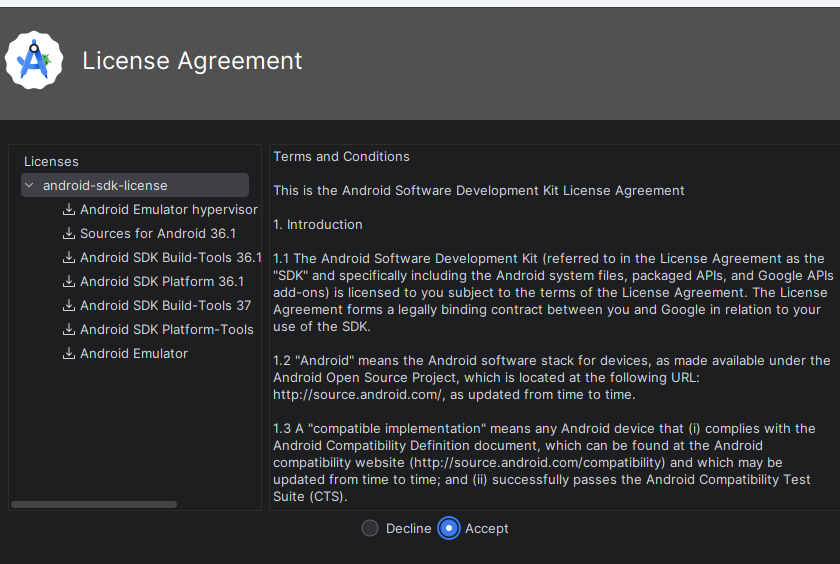
\includegraphics[width=\linewidth]{img/installSDK1.png}
  \captionof{anexofloat}{SDK Manager -- selección del Android SDK}
\end{minipage}
\hfill
\begin{minipage}[t]{0.47\textwidth}
  \centering
  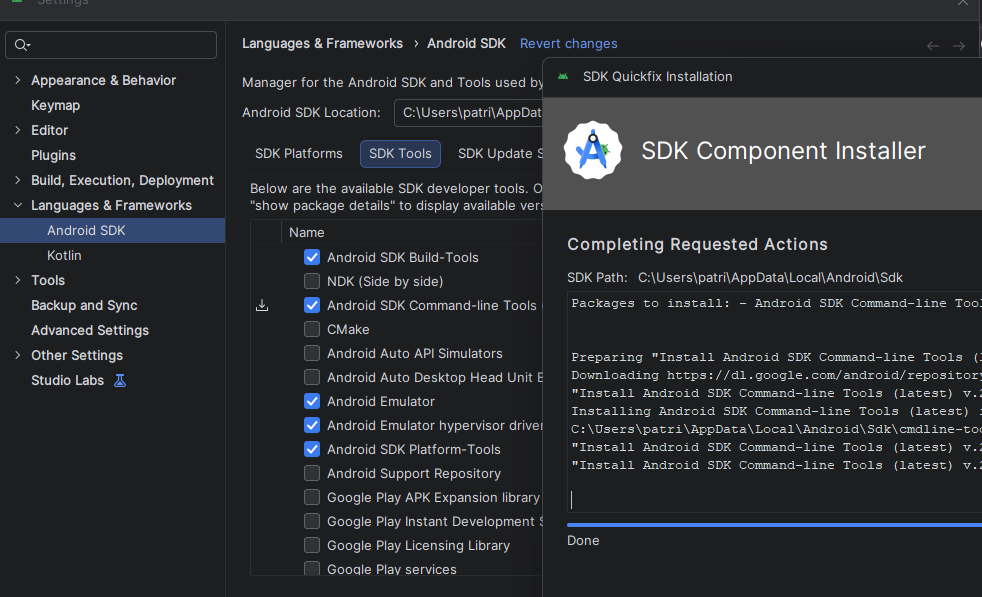
\includegraphics[width=\linewidth]{img/installComponents.png}
  \captionof{anexofloat}{Instalación de Command-line Tools}
\end{minipage}

\vspace{1.2cm}

\noindent
\begin{minipage}[t]{0.47\textwidth}
  \centering
  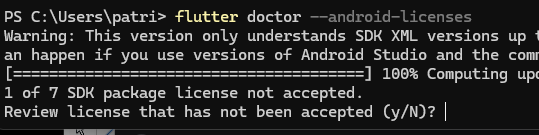
\includegraphics[width=\linewidth]{img/ActivacionLicenciaFlutter.png}
  \captionof{anexofloat}{Activación de licencias del Android SDK}
\end{minipage}
\hfill
\begin{minipage}[t]{0.47\textwidth}
  \centering
  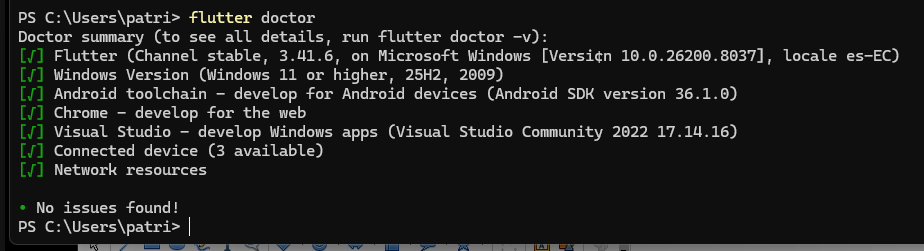
\includegraphics[width=\linewidth]{img/ComprobacionEntornoNecesarioParaFlutter.png}
  \captionof{anexofloat}{Verificación final con \texttt{flutter doctor}}
\end{minipage}

\end{document}
